\begin{pastexam}[label={px:ntu-111-dsaa-07}]{臺大資工所 111 學年度 第 7 題}
（單選）

(5 points) In a \textit{max-heap} stored in an array, after these 6 numbers have been inserted in this
exact sequence: 5, 4, 2, 6, 1, 3, what is the value of the node at index 2 (with the root being
the node at index 1)?
\begin{enumerate}[label=(\Alph*)]
\item 1
\item 2
\item 4
\item 5
\item none of the other choices
\end{enumerate}
\end{pastexam}

\begin{pastsoln}
答案是 (D) 5。

「依序插入」指從空堆積開始，每次用
\proc{Max-Heap-Insert}：放在陣列最後一格，再和父節點比，比父節點大就交換、往上爬
（資結書第~8.1~節、虛擬碼~8.2）。 索引 $i$ 的父節點是 $\lfloor i/2 \rfloor$。
\begin{center}
\begin{tabular}{cll}
\toprule
插入 & 過程 & 陣列 $A[1..]$ \\
\midrule
5 & 放在 $A[1]$ & $5$ \\
4 & 放在 $A[2]$，父 $A[1] = 5$ 較大，停 & $5, 4$ \\
2 & 放在 $A[3]$，父 $5$ 較大，停 & $5, 4, 2$ \\
6 & 放在 $A[4]$；$6 > A[2] = 4$，交換；$6 > A[1] = 5$，交換 & $6, 5, 2, 4$ \\
1 & 放在 $A[5]$，父 $A[2] = 5$ 較大，停 & $6, 5, 2, 4, 1$ \\
3 & 放在 $A[6]$；$3 > A[3] = 2$，交換；父 $A[1] = 6$ 較大，停 & $6, 5, 3, 4, 1, 2$ \\
\bottomrule
\end{tabular}
\end{center}
最後的堆積畫成樹：
\begin{center}
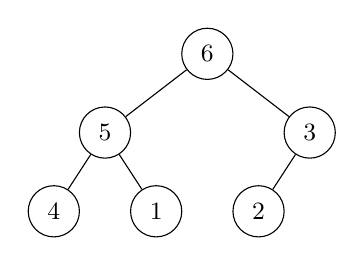
\begin{tikzpicture}[level distance=10mm,
  level 1/.style={sibling distance=26mm}, level 2/.style={sibling distance=13mm},
  every node/.style={circle,draw,minimum size=6.5mm,inner sep=0pt,font=\small}]
\node {6}
  child {node {5} child {node {4}} child {node {1}}}
  child {node {3} child {node {2}} child[missing]};
\end{tikzpicture}
\end{center}
索引 $2$ 的節點是 $5$，選 (D)。 (C) 4 是插入 6 之前 $A[2]$ 的值，6 往上爬時把 4 換到了 $A[4]$。
(A) 1 在 $A[5]$，(B) 2 在 $A[6]$。

如果改成先把六個數放進陣列再 \proc{Build-Max-Heap}，結果是 $6, 5, 3, 4, 1, 2$，這組資料剛好
一樣；但題目明說「依序插入」，照插入來做。
\end{pastsoln}
